% Editable native annotations around unchanged verified IDE photographs.
\par
\begin{figure}[htbp]
  \centering
  \sbox0{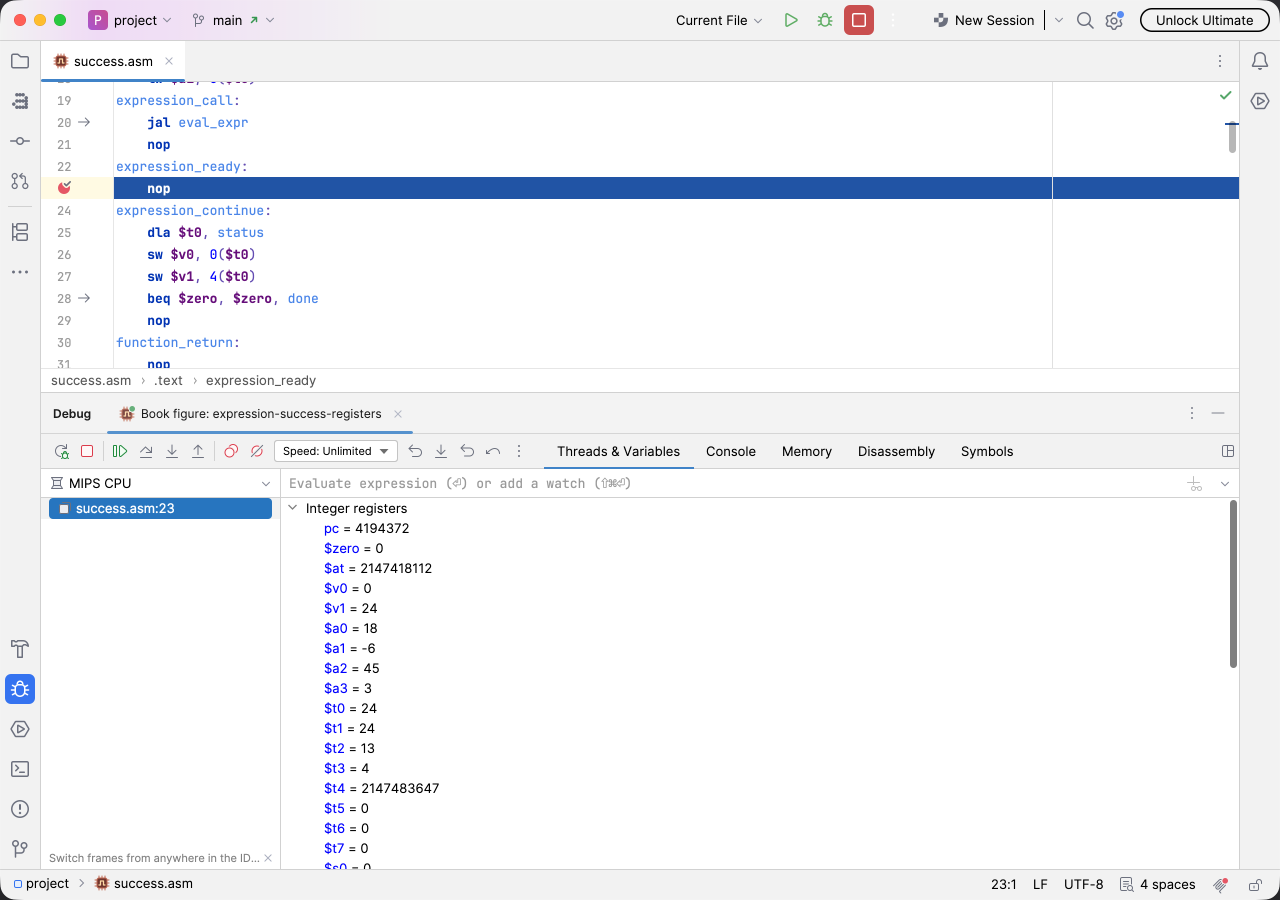
\includegraphics[artifact]{packages/017-expression-evaluator/captures/f01/registers.png}}
  \sbox2{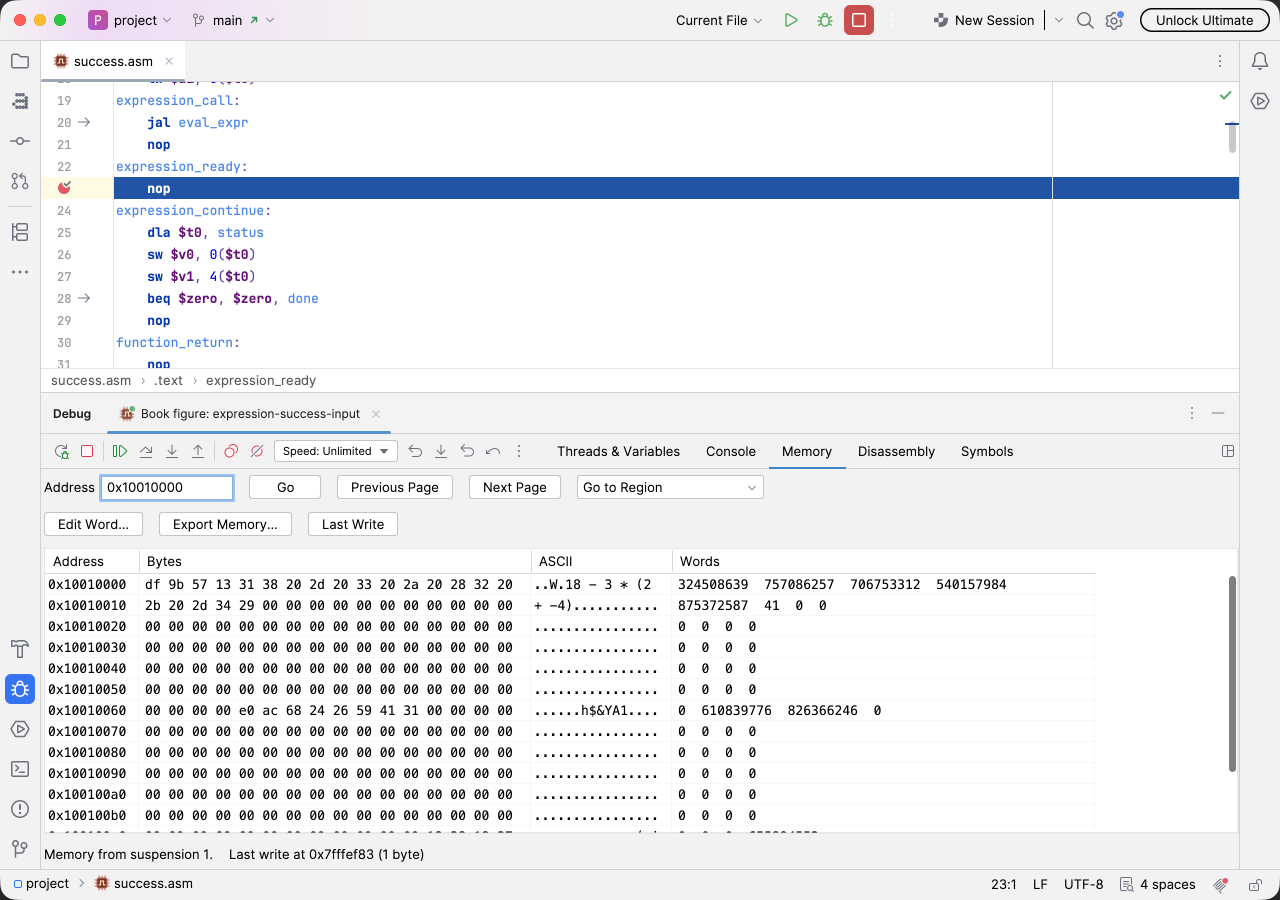
\includegraphics[artifact]{packages/017-expression-evaluator/captures/f01/input.png}}
  \sbox4{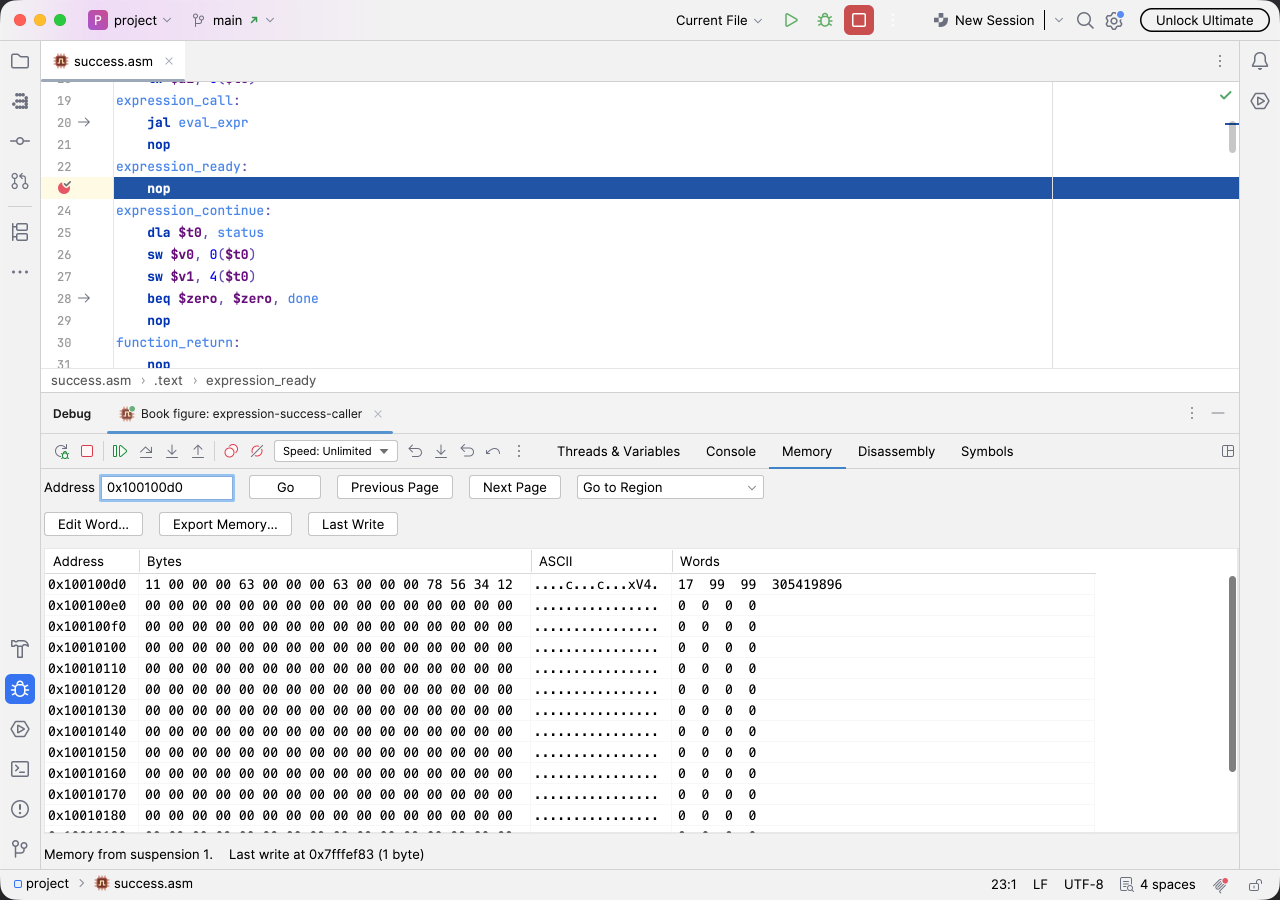
\includegraphics[artifact]{packages/017-expression-evaluator/captures/f01/caller.png}}
  \edef\MARSexpressionsuccesssourceLeft{\the\dimexpr0.036718750\wd0\relax}
  \edef\MARSexpressionsuccesssourceBottom{\the\dimexpr0.774444444\ht0\relax}
  \edef\MARSexpressionsuccesssourceRight{\the\dimexpr0.713281250\wd0\relax}
  \edef\MARSexpressionsuccesssourceTop{\the\dimexpr0.147777778\ht0\relax}
  \edef\MARSexpressionsuccessregistersLeft{\the\dimexpr0.246093750\wd0\relax}
  \edef\MARSexpressionsuccessregistersBottom{\the\dimexpr0.312222222\ht0\relax}
  \edef\MARSexpressionsuccessregistersRight{\the\dimexpr0.553906250\wd0\relax}
  \edef\MARSexpressionsuccessregistersTop{\the\dimexpr0.640000000\ht0\relax}
  \edef\MARSexpressionsuccessinputLeft{\the\dimexpr0.034375000\wd2\relax}
  \edef\MARSexpressionsuccessinputBottom{\the\dimexpr0.311111111\ht2\relax}
  \edef\MARSexpressionsuccessinputRight{\the\dimexpr0.584375000\wd2\relax}
  \edef\MARSexpressionsuccessinputTop{\the\dimexpr0.608888889\ht2\relax}
  \edef\MARSexpressionsuccesscallerLeft{\the\dimexpr0.034375000\wd4\relax}
  \edef\MARSexpressionsuccesscallerBottom{\the\dimexpr0.334444444\ht4\relax}
  \edef\MARSexpressionsuccesscallerRight{\the\dimexpr0.584375000\wd4\relax}
  \edef\MARSexpressionsuccesscallerTop{\the\dimexpr0.608888889\ht4\relax}
  \begin{tikzpicture}[alt={Four annotated details at expression return for 18 - 3 * (2 + -4). Native signed status is zero and result is 24. The unchanged seventeen-byte input begins at 0x10010004 after its guard and spans two memory rows. A separate caller-memory row shows length seventeen and both result words still 99 before publication.}]
    \node[anchor=north west,inner sep=0,font=\small\bfseries] (source-title) at (6mm,0) {Next instruction after return};
    \node[anchor=north west,inner sep=0] (source) at ([yshift=-1mm]source-title.south west) {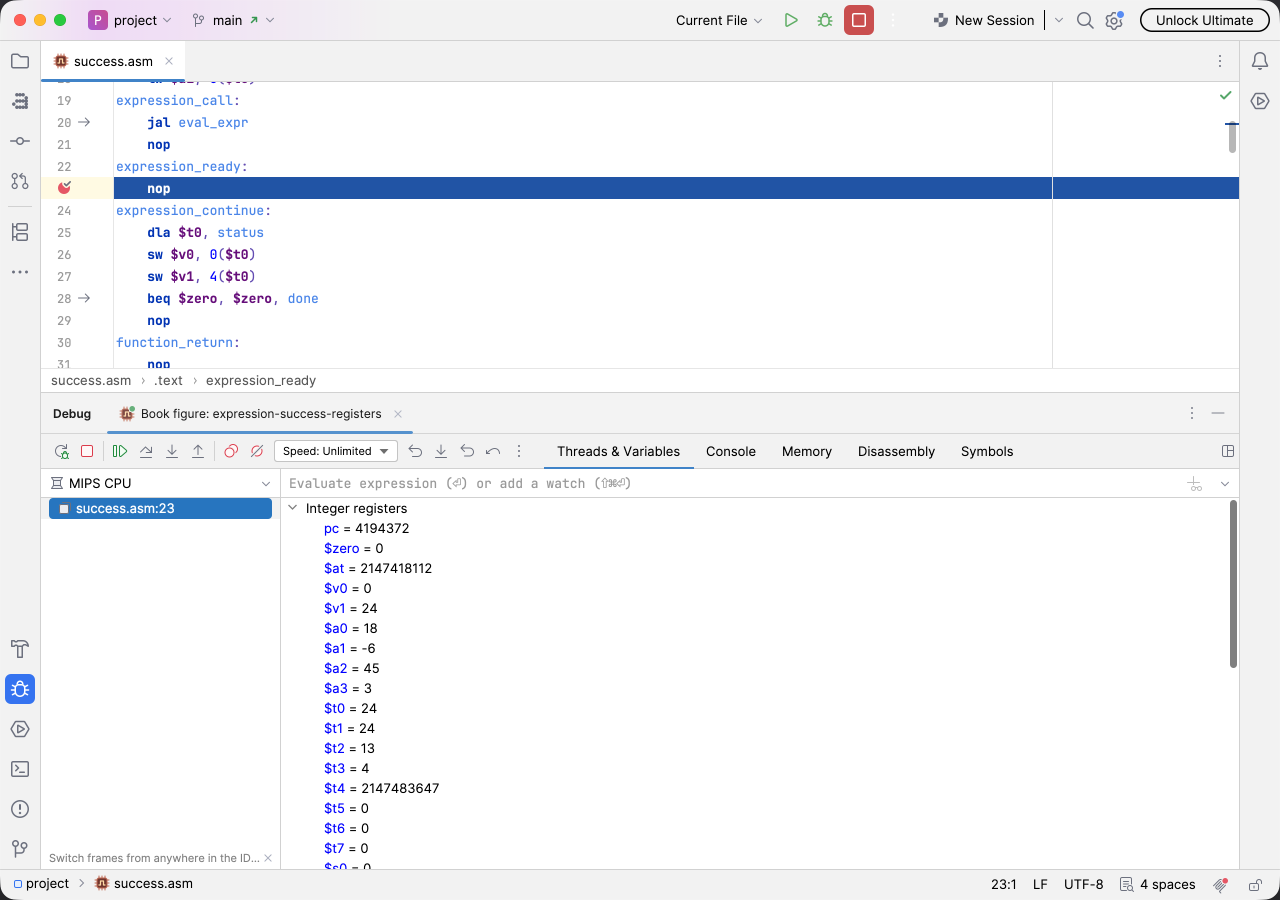
\includegraphics[width=0.54\linewidth,artifact,trim={\MARSexpressionsuccesssourceLeft{} \MARSexpressionsuccesssourceBottom{} \MARSexpressionsuccesssourceRight{} \MARSexpressionsuccesssourceTop{}},clip]{packages/017-expression-evaluator/captures/f01/registers.png}};
    \begin{scope}[shift={(source.south west)},x={($(source.south east)-(source.south west)$)},y={($(source.north west)-(source.south west)$)}]
      \draw[black,line width=0.7pt] (0.215625000,0.057142857) rectangle (0.384375000,0.371428571);
      \node[draw=black,fill=white,circle,inner sep=1.5pt,font=\footnotesize] at ($(0.215625000,0.371428571)+(-3mm,0)$) {1};
    \end{scope}
    \node[anchor=north west,inner sep=0,font=\small\bfseries] (registers-title) at (0.58\linewidth,0 |- source-title.north) {Signed return values};
    \node[anchor=north west,inner sep=0] (registers) at ([yshift=-1mm]registers-title.south west) {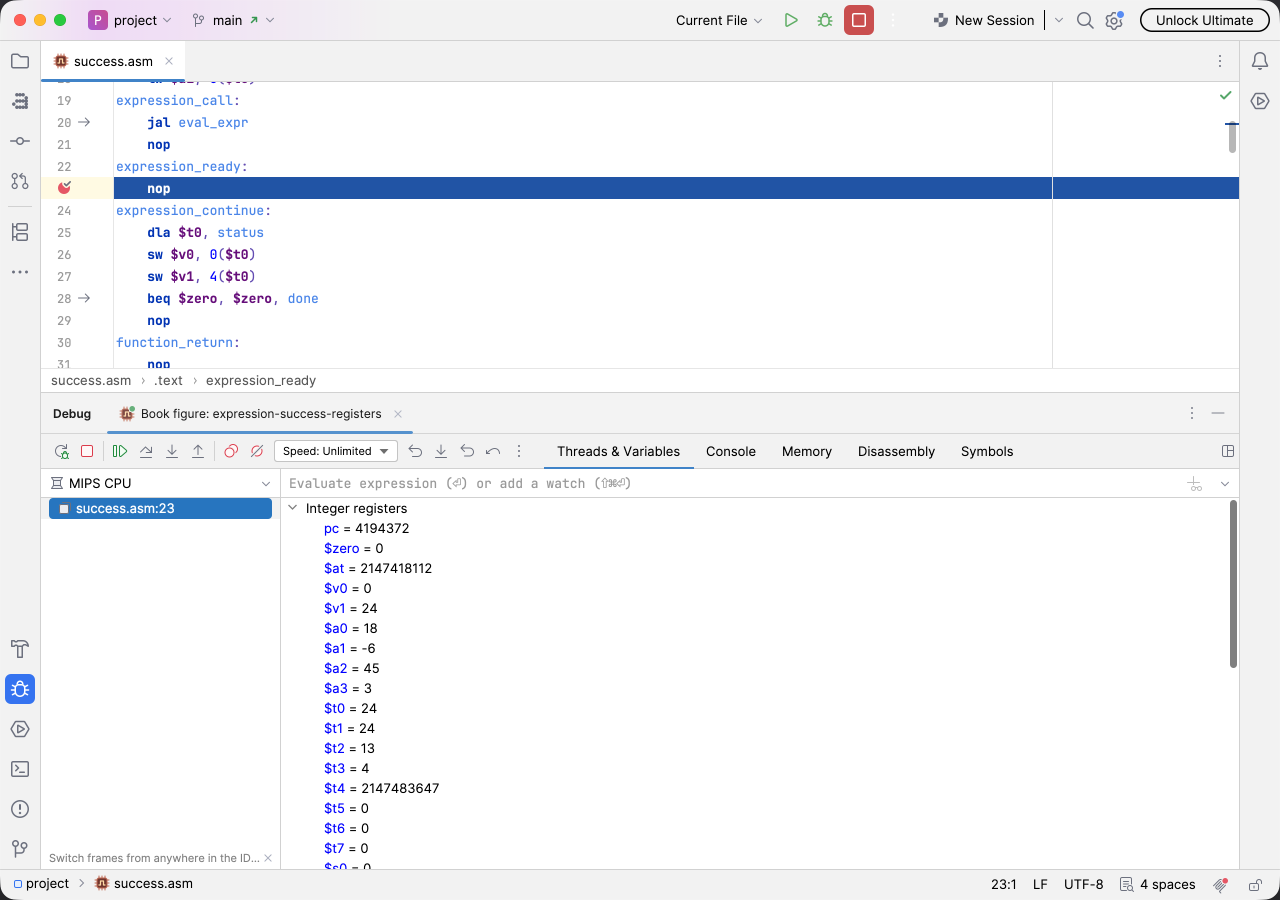
\includegraphics[width=0.42\linewidth,artifact,trim={\MARSexpressionsuccessregistersLeft{} \MARSexpressionsuccessregistersBottom{} \MARSexpressionsuccessregistersRight{} \MARSexpressionsuccessregistersTop{}},clip]{packages/017-expression-evaluator/captures/f01/registers.png}};
    \begin{scope}[shift={(registers.south west)},x={($(registers.south east)-(registers.south west)$)},y={($(registers.north west)-(registers.south west)$)}]
      \draw[black,line width=0.7pt] (0.023437500,0.023255814) rectangle (0.250000000,0.953488372);
      \node[draw=black,fill=white,circle,inner sep=1.5pt,font=\footnotesize] at ($(0.023437500,0.953488372)+(-3mm,0)$) {2};
    \end{scope}
    \node[anchor=north west,inner sep=0,font=\small\bfseries] (input-title) at ([yshift=-3mm]source.south west) {Input bytes, preceding guard and mapped padding};
    \node[anchor=north west,inner sep=0] (input) at ([yshift=-1mm]input-title.south west) {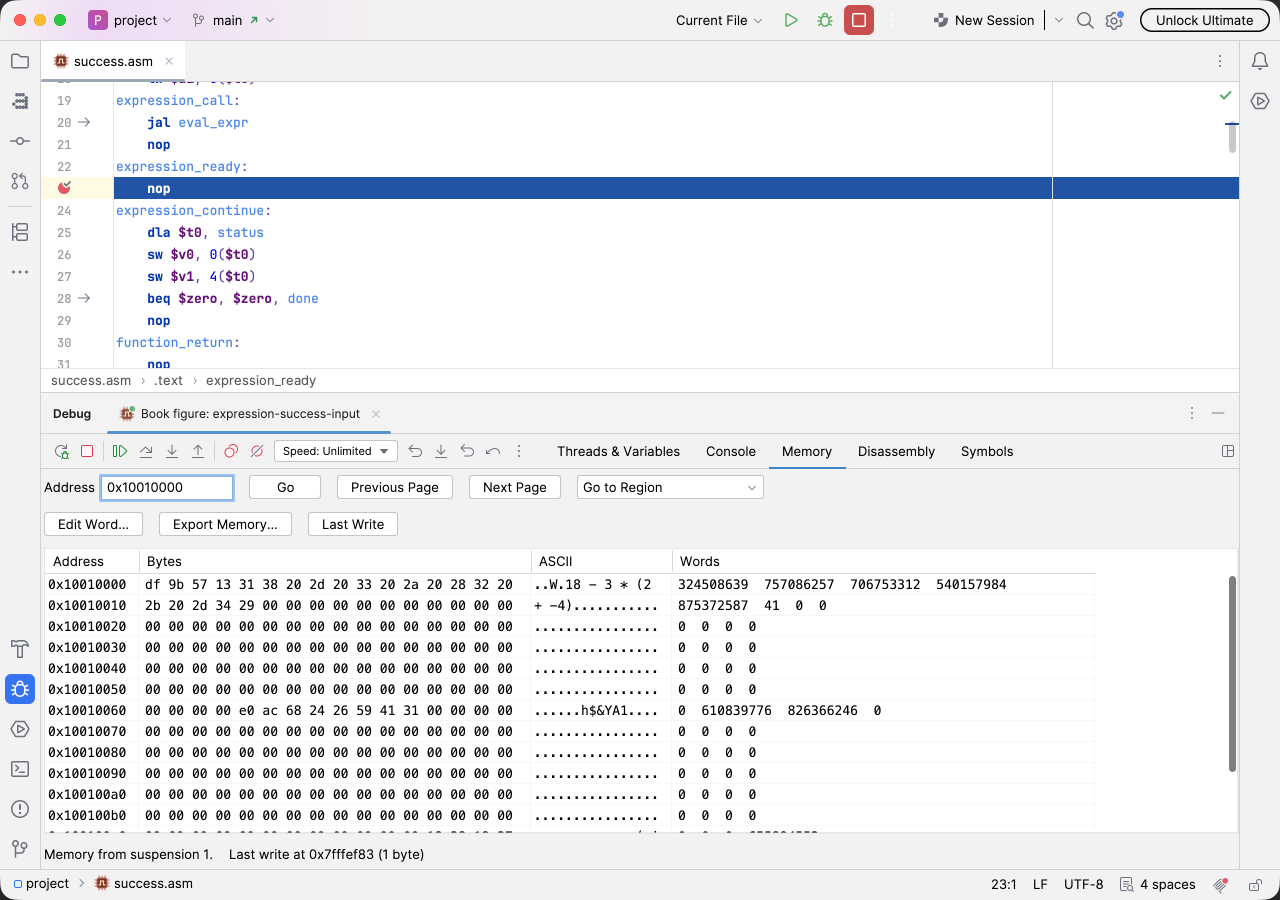
\includegraphics[width=0.84\linewidth,artifact,trim={\MARSexpressionsuccessinputLeft{} \MARSexpressionsuccessinputBottom{} \MARSexpressionsuccessinputRight{} \MARSexpressionsuccessinputTop{}},clip]{packages/017-expression-evaluator/captures/f01/input.png}};
    \begin{scope}[shift={(input.south west)},x={($(input.south east)-(input.south west)$)},y={($(input.north west)-(input.south west)$)}]
      \draw[black,line width=0.7pt] (0.194672131,0.055555556) rectangle (0.997950820,0.638888889);
      \node[draw=black,fill=white,circle,inner sep=1.5pt,font=\footnotesize] at ($(0,0.638888889)+(-3mm,0)$) {3};
    \end{scope}
    \node[anchor=north west,inner sep=0,font=\small\bfseries] (caller-title) at ([yshift=-3mm]input.south west) {Caller length and unpublished result words};
    \node[anchor=north west,inner sep=0] (caller) at ([yshift=-1mm]caller-title.south west) {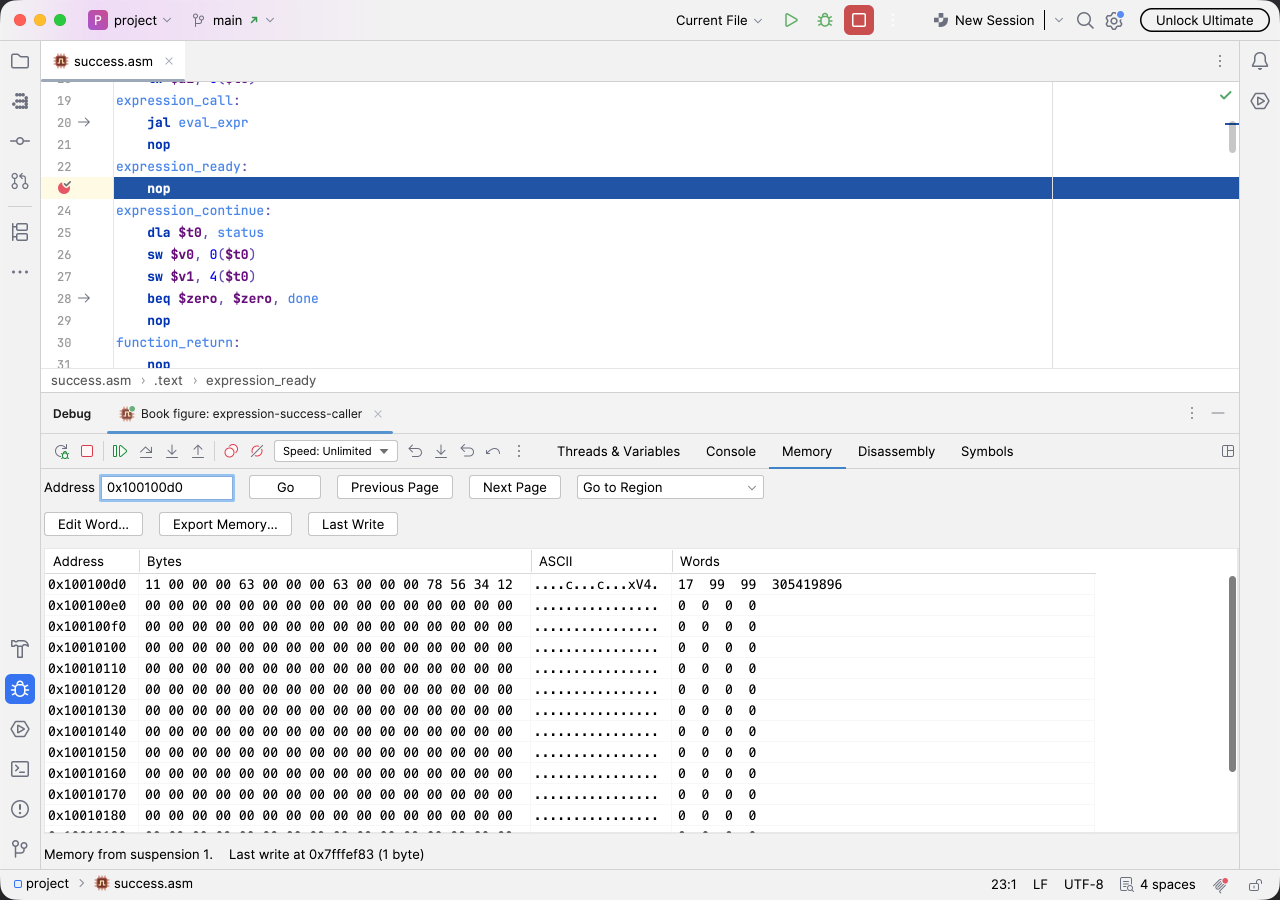
\includegraphics[width=0.84\linewidth,artifact,trim={\MARSexpressionsuccesscallerLeft{} \MARSexpressionsuccesscallerBottom{} \MARSexpressionsuccesscallerRight{} \MARSexpressionsuccesscallerTop{}},clip]{packages/017-expression-evaluator/captures/f01/caller.png}};
    \begin{scope}[shift={(caller.south west)},x={($(caller.south east)-(caller.south west)$)},y={($(caller.north west)-(caller.south west)$)}]
      \draw[black,line width=0.7pt] (0.194672131,0.078431373) rectangle (0.997950820,0.490196078);
      \node[draw=black,fill=white,circle,inner sep=1.5pt,font=\footnotesize] at ($(0,0.490196078)+(-3mm,0)$) {4};
    \end{scope}
  \end{tikzpicture}
  \par\smallskip
  \begin{minipage}{\linewidth}
    \small
    \begin{enumerate}
      \setlength{\itemsep}{2pt}
            \setlength{\parsep}{0pt}
      \item The blue \texttt{nop} at \texttt{expression\_ready} is next after \texttt{eval\_expr} returns. This stop precedes the caller\textquotesingle s result stores. Read \texttt{\$v0} first: the meaning of \texttt{\$v1} depends on that status.
      \item \texttt{\$v0 = 0} means success, so \texttt{\$v1 = 24} is the expression value. Unary minus gives $-4$; the group gives $2+(-4)=-2$; multiplication gives $3\cdot(-2)=-6$; subtraction gives $18-(-6)=24$. The grouped expression and multiplication supply successful operands before the outer subtraction is checked.
      \item The slice begins at \texttt{0x10010004}, four bytes into the first row. Its seventeen bytes encode \texttt{18 - 3 * (2 + -4)}; spaces count toward positions. Bytes \texttt{2b 20 2d 34 29} on the second row are the final \texttt{+ -4)}. The preceding guard and following mapped zeros are outside the supplied slice. The complete data image remains unchanged, and every evaluator input read fits the slice.
      \item The row at \texttt{0x100100d0} contains length, caller status, caller second result, and the final guard. Bytes \texttt{63 00 00 00} encode decimal 99, the initial value of both result words. The evaluator returns through registers and leaves caller data read-only. Continuing past \texttt{expression\_continue} lets the caller replace those two words; exit later reuses \texttt{\$v0} for its service number. Here length is \texttt{11 00 00 00}, hexadecimal \texttt{0x11}, or decimal 17. The live register result 24 and the stored sentinel 99 describe different points in the caller\textquotesingle s execution.
    \end{enumerate}
  \end{minipage}
  \caption{Precedence and unary negation produce the value 24 from the seventeen-byte input.}
  \label{capture:017-expression-evaluator-f01}
  \label{expression-f01}
\end{figure}
\par
